\chapter{Limits of ADC figure of merit}\label{sc:limits}
Efficiency is one of the key measures of analog-to-digital
converters. A more efficient
ADC can translate into longer battery life of our
hand-held devices. For ADCs the power dissipation ($P$), sampling frequency
($f_s$) and effective number of bits ($B$) are combined to give a
single measure of the efficiency, the figure of merit (FOM). 
For the
figures of merit discussed here a smaller value is better. 

The
historic figure of merit proposed by Walden \cite{walden99}
was \req{fomwalden}\footnote{It was actually presented as $FOM =2^Bf_s/P$, but the
  inverse is the most used.}
  \begin{equation}
    \label{eq:fomwalden}
    FOM = \dfrac{P}{2^{B}f_s}
  \end{equation}
This FOM, however, is incorrect if we assume the ADCs should be limited by
thermal noise. A more correct figure of merit is
  \begin{equation}
    \label{eq:fom}
    FOM = \dfrac{P}{2^{2B}f_s}
  \end{equation}

This figure of merit, the Thermal FOM, is based on the fact that in an
ADC limited by thermal noise we must use 4 times the power if we add
one bit of resolution, since the required sampling capacitance increases 4 times. A more
in-depth argument is given in \cite{schreier.uds} on page 360. 

If we have the ADC parameters (accuracy, power dissipation, speed) we
can calculate the FOM from \req{fom}. But
what is the limit of the FOM? How low FOM can we expect to get with
future ADCs? 

We will in this chapter derive expressions for the FOM
limit and compare the limit to results of published ADCs. But first 
we have to derive the required sampling
capacitance for a certain resolution.


\section{Required sampling capacitance}
We assume a switched-capacitor based ADC. The input signal is sampled
across a sampling capacitor ($C$). And $C$ is the only capacitor in
the ADC. In such a system the thermal noise
power can be represented as
\begin{equation}
\label{eq:thermal}
\overline{V_{thermal}^2} = a_1\times k T/C  
\end{equation}
where $a_1$ is a constant greater than one, $k$ is Boltzmann's constant, $T$ is the temperature
in Kelvin and $C$ is the sampling capacitance.

 The thermal noise power should be less
than the quantization noise power, but not too small, because a 
small thermal noise power will cost in terms of power dissipation. 
We assume that the quantization noise power is four times the thermal noise power.
\begin{equation}
  \label{eq:lsbvsthermal}
  \overline{V_{LSB}^2} = 4\times\overline{V_{thermal}^2}
\end{equation}
where $\overline{V_{LSB}^2}$ is the quantization noise power, which can
be calculated as
\begin{equation}
\label{eq:lsb}
\overline{V_{LSB}^2} = V_{LSB}^2/12= V_{PP}^2/(2^{2B}\times
  12)
\end{equation}
where $V_{LSB}$ is the voltage step of the least significant bit (LSB)
and  $V_{PP}$ is the peak-to-peak
input signal voltage.

If we combine \req{thermal}, \req{lsbvsthermal} and \req{lsb} we get
\begin{equation} 
  \label{eq:cap1}
 \dfrac{ V_{PP}^2}{2^{2B}\times12} = 4 \times a_1 \times kT/C
\end{equation}

Solved for sampling capacitance ($C$) \req{cap1} becomes
\begin{equation}
\label{eq:cap}
C = a_1 \times \dfrac{48 k T 2^{2B}}{V_{PP}^2}  
\end{equation}

Using equation \req{cap} we can calculate how large $C$ must be for a certain  resolution. For example
for $V_{PP} = 1\:V, T = 300\:K$ we get $C_{[B=6]} = 0.8fF$, $ C_{[B=12]}  =
3.3pF$, and $C_{[B=14]} = 53pF$. 

Assume the capacitor is used in a switched capacitor circuit, and that
 an amplifier is used to charge the capacitor to its final value.
We will consider two methods for this capacitance to reach its final
value: a constant ramp, and linear settling. Constant ramp is 
equivalent to what is used in comparator-based switched-capacitor
circuits. Linear settling is equivalent to what is used
in opamp based switch-capacitor circuits and open-loop residue
amplifiers. 

\section{Constant ramp FOM limit}
For a constant ramp the voltage across $C$ is given by
\begin{equation}
\label{eq:const1}
V_o(t) = \dfrac{I}{C}\times t 
\end{equation}
where $t = 1/2f_s$, $I$ is the current used to charge the capacitor,
and $f_s$ is the sampling frequency.

 The maximum 
$V_o(t)$ is equal to $V_{PP}$, and will require the most time. Accordingly, we
set $V_o(t) = V_{PP}$, insert for \req{cap} in \req{const1}, and
multiply each side with $V_{DD}$ 
\begin{equation}
\label{eq:const2}
  V_{PP}V_{DD} = \dfrac{I V_{DD} V_{PP}^2}{96 a_1 k T 2^{2B} f_s}
\end{equation}  
Solved for FOM \req{const2} becomes
\begin{equation}
\label{eq:ramp}
  FOM_{ramp} = \dfrac{P}{2^{2B}f_s} = \dfrac{96 a_1 kT }{\dfrac{V_{PP}}{V_{DD}}}
\end{equation}
 This FOM does not depend on the number of bits
($B$) or the sampling frequency ($f_s$).

\section{Linear settling FOM limit}
We assume the voltage across $C$ must reach a final value within a certain accuracy,
given by the LSB, and reach this accuracy
within half the sampling period
($1/2f_s$). 

Assume a transconductance amplifier (an ideal transistor with
resistive load $R_o = 1/g_m$) is used to drive the capacitance
$C$. The amplifier has the transfer function
\begin{equation}
  \dfrac{V_o(s)}{V_i(s)} = \dfrac{1}{1 + s C/g_m}
\end{equation}
 where $V_o$ is the voltage across the capacitance, $V_i$ is the
 input signal voltage, and $g_m$ is the
 transconductance.

Assume the input is a unit step function $V_i(t) = V_{PP}u(t)$. The
output will then be
\begin{equation}
V_o(t) = V_{PP}-V_{PP}e^{-g_m t /C}, t > 0
\end{equation}

Written in terms of the settling error ($\epsilon = V_{PP} -
V_o(t)$) we get
\begin{equation}
\label{eq:epsi}
\epsilon = V_{PP} e^{- g_m t/C }
\end{equation}

The settling error ($\epsilon$) should be smaller than one LSB,
$\epsilon < V_{PP}/2^B$, but to simplify we set $\epsilon = LSB$. The transconductance in \req{epsi} can be written as $g_m =
  \eta_1 2 I_D/V_{EFF}$  where $\eta_1$ is a technology dependent
  constant (it depends on high field effects and short channel
  effects, $\eta_1$ is larger than zero, but less than one. For a 90nm
  process it's around 0.5-0.6), $I_D$ is the
  drain current and $V_{EFF}$ is the effective gate
  overdrive. Inserted into \req{epsi} together with \req{cap} results in
\begin{equation}
\dfrac{V_{PP}}{2^B} =V_{PP} \: e^{\left(-\dfrac{\eta_1 2 I_D
    \dfrac{V_{PP}^2}{V_{DD}^2}V_{DD}^2}{2f_s\dfrac{V_{EFF}}{V_{DD}}V_{DD}a_148kT2^{2B}}\right)}
\end{equation}
Solved for FOM we get
\begin{equation}
\label{eq:settling}
FOM = \dfrac{I_DV_{DD}}{2^{2B}f_s} = \dfrac{ B \ln(2)
  \dfrac{V_{EFF}}{V_{DD}}}{\eta_1 \dfrac{V_{PP}^2}{V_{DD}^2}} a_1 48kT
\end{equation}
According to this equation, it will be more difficult to
get a good figure of merit  with additional bits, but this ignores the influence
of parasitic capacitances.

\section{FOM limit including parasitic capacitance}
Assume that an ADC has as many stages as bits ($B$), define $M_0$ as
the number of circuit nodes per
stage and $C_0$ as the parasitic capacitance per node. The total
parasitic capacitance in the ADC will then be
\begin{equation}
\label{eq:cap_p}
C_p = C_0 M_0 B  
\end{equation} 

The parasitic capacitance \req{cap_p} will add to the load of our
transconductance amplifier, accordingly the load will be
\begin{equation}
\label{eq:parcap}
C = a_1 \times \dfrac{48 k T 2^{2B}}{V_{PP}^2} + C_0 M_0 B
\end{equation}
Inserted into \req{epsi} %with some manipulation gives
\begin{equation}
\dfrac{V_{PP}}{2^B} =V_{PP} \:e^{\left(-\dfrac{\eta_1 2
    I_D}{2f_s\dfrac{V_{EFF}}{V_{DD}}V_{DD}}\dfrac{1}{\dfrac{a_148kT2^{2B}}{V_{PP}^2}+
  C_0 M_0 B}\right)}
\end{equation}
And with some manipulation
\begin{equation}
\label{eq:parfom}
FOM = \dfrac{B \ln(2) \dfrac{V_{EFF}}{V_{DD}}}{\eta_1
  \dfrac{V_{PP}^2}{V_{DD}^2}}\left( a_1 48 kT + \dfrac{C_0 M_0 B
    V_{PP}^2}{2^{2B}}\right)
\end{equation}
For $C_0 = 0$ \req{parfom} reduces to \req{settling}. 

These three 
equations: \req{ramp}, \req{settling}, and \req{parfom}, are based on numerous
assumptions, and it is interesting to see how well the equations predict
published results for ADCs.

\section{Comparison with published results}
The FOM limits have been compared to selected ADCs published in Journal of
Solid State Circuits (JSSC) in the 
years 1975-2008.\footnote{The data for this study can be downloaded
  from \url{http://www.wulff.no/carsten} \textit{Electronics},
  \textit{ADC FOM}} And selected ADCs published at the International Solid State 
Circuits Conference (ISSCC) in the years 2000-2008. 

The comparison is
shown in Fig. \ref{fig:fomadcs}. We have used
$V_{EFF}/V_{DD} = 1/8, V_{PP}/V_{DD} = 0.5, \eta_1 = 0.5, a_1 = 1,
T = 300\: K$. Choosing the value for $M_0$ and $C_0$ is guesswork since
they depend on ADC architecture and technology, but it
is unlikely that $M_0 < 10$ and $C_0 < 1fF$. A more realistic model
would arguably be $M_0 = 200$ and $C_0 = 10fF$.  

None of the published
ADCs go below the FOM limit given by \req{settling} or \req{ramp}, but for high number of bits ($>$ 14-bits)
they begin to approach the limit. At high number of bits it is more
straightforward to achieve a good FOM because the required
sampling capacitor becomes large and the parasitic capacitances become
less important. But for low to medium number of bits ($<$ 12-bits) the
required sampling capacitance is so low ($<$ 4 pF)  that the parasitic
capacitances dominate. 

At 7-bit the best ADC is more
than 100 times worse than the FOM limit. 

The parasitic FOM limit given by \req{parfom} match the shape of the
data points. 
The realistic model ($M_0 = 200, C_0 = 10fF$) enclose most of the data
points, and the likely limit ($M_0 = 10, C_0 = 1fF$) enclose all.


%The
%four points between the two parasitic FOM limit lines are from ISSCC 2008, where a special
%session was held for high efficiency ADCs. These four ADCs are 10
%times better than the rest of their class. 

For ENOB larger than six bits constant ramp has an advantage over
linear settling.


\begin{figure}[htb]
\centering 
 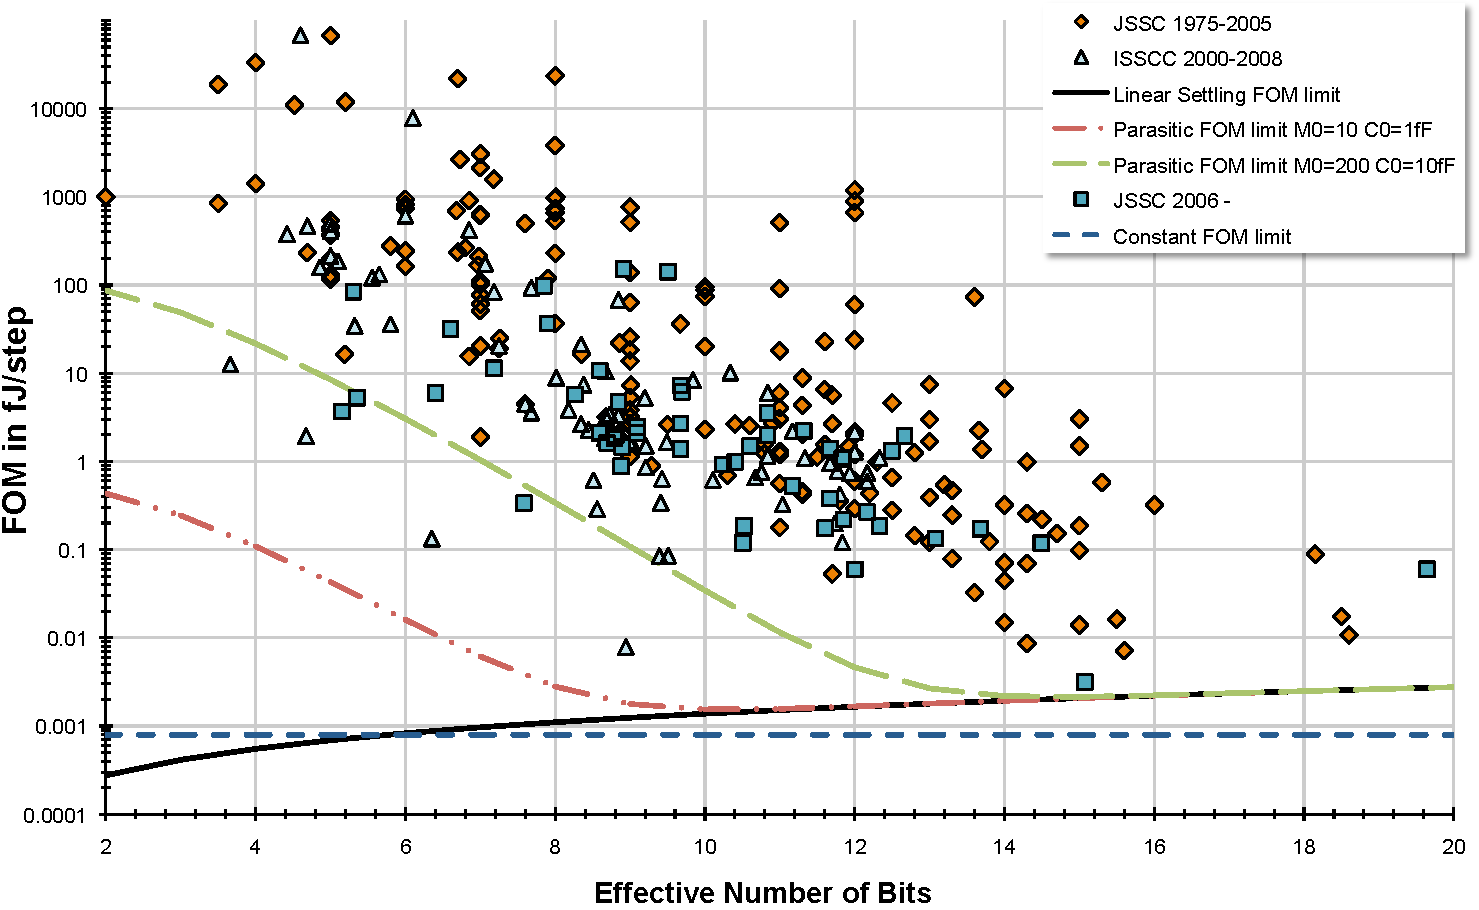
\includegraphics[width=\myfigwidthl]{graphics/adcfom}
  \caption{FOM versus bits for selected ADCs published in JSSC in the
  years 1975-2008 and ADCs published at ISSCC 2000-2008 compared to:
  the FOM limit for constant ramp, FOM limit for linear settling, and the parasitic FOM model}
  \label{fig:fomadcs}
\end{figure}


%%% Local Variables: 
%%% mode: latex
%%% TeX-master: "../../wulff/work/ntnu/phd/thesis/tb_limits"
%%% End: 
